\chapter{Normalisation}

Une des difficultés de la discipline des ``réseaux informatiques '' réside dans la quantité, que certains trouveront abusive, des sigles, normes, organismes de normalisation\ldots Il est toutefois nécessaire d'intégrer cette terminologie, d'apprendre ce langage, pour mieux apréhender ce `` nouveau monde ''. Le meilleur conseil que nous pouvons donner à l'étudiant est de se procurer un dictionnaire de téléinformatique/télécommunications.

\section{Définition et utilité de la normalisation}

Pour comprendre la normalisation, essayez de lire le mot suivant: yfgtke

Impossible si vous ne connaissez pas les règles de représentation des mots. En effet, si des normes d'écriture n'avaient pas été établies, il aurait été difficile de communiquer par ce moyen. Donc, la normalisation n'est rien d'autre que des règles établies qui doivent être suivies par les entités désirant communiquer.

Au fait, le mot était rectangle.

Evidemment, si chacun établit et suit sa propre norme, la normalisation ne sert à rien. C'est pourquoi la normalisation n'a d'intérêt que si elle est appliquée par une grande communauté.

Le dictionnaire donne la signification suivante:

\begin{itemize}
	\item normalisation: assujettissement à des normes, des types, des règles techniques;
	\item norme: principe, règle,type, modèle.
\end{itemize}

Les constructeurs informatiques et les opérateurs de télécommunications ont été les premiers à établir des normes dans ce domaine. Des normes multiples et incompatibles coexistent. Des passerelles sont établies entre certaines normes.

\section{Les principaux organismes de normalisation}
Dans ce paragraphe, nous allons présenter quelques organismes de normalisation parmi les plus importants. Certains de ces organismes s'intéressent à la normalisation dans différents domaines, dont celui des télécommunications; d'autres organismes (indiqués avec une astérixe)sont issus des opérateurs de télécommunications. Pour bien les positionner, nous utiliserons le critère de portée administratif et légal. Ainsi, nous distinguons:

\begin{itemize}
	\item les organismes internationaux: ISO, ITU (ex-CCITT);
	\item les organismes multi-nationaux (Europe): CEN/CENELEC, ETSI;
	\item les organismes nationaux: AFNOR (FR), ANSI (USA), DIN (GER), BSI (UK), Telecoms;
\end{itemize}
\begin{figure}[H]
	\centering
	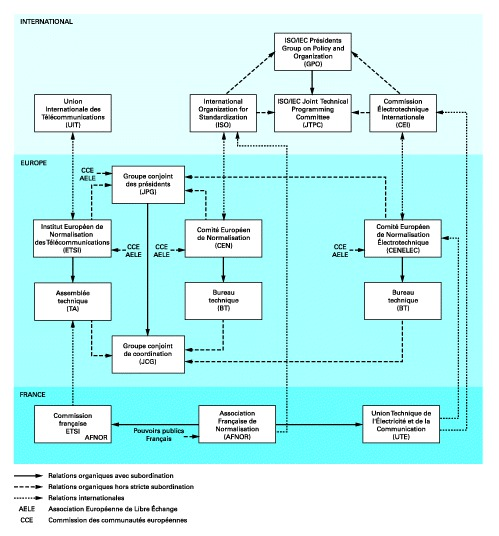
\includegraphics{partie1/normalisation.jpg}
\end{figure}
Certains organismes privés essentiellement américains ont un très grand poids:
\begin{itemize}
	\item DARPA du DoD;
	\item IEEE;
	\item EIA;
	\item NBS;
	\item ECMA;
	\item \ldots
\end{itemize}

Voilà un exemple de standards pour le sans-fil :
\begin{figure}[H]
	\centering
	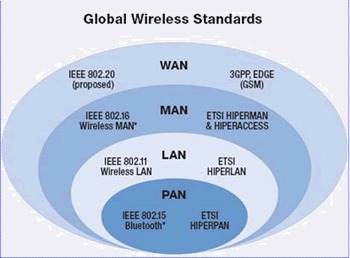
\includegraphics{partie1/standardsexemple.jpg}
\end{figure}



